\documentclass[12pt]{article}
\usepackage{graphicx}
  
%
\title{EE 230: Analog Circuits Lab\\ Lab No. 2\\ OpAmp based feedback Lab}
% Author[Enter details of author here]
\author{Anupam Rawat, 22b3982}
\date{January 12, 2024}


\begin{document}
\maketitle

\section{OpAmp based Negative feedback circuits}

\addcontentsline{toc}{section}{Unnumbered Section}
\section*{(a) Inverting Amplifier}
\subsection*{a.1 Aim of the experiment}
Analyse a negative feedback circuit using an Op-Amp and study the effect of negative feedback on the gain of the circuit.

\subsection*{a.2 Design}
The design consists of an OpAmp with a feedback resistor connected between the output and the inverting input of the OpAmp and the input voltage is connected to the inverting input of the OpAmp. The gain of the circuit is given by the equation:
 \begin{equation}
     V_{out} = V_{in} \cdot (1 + \frac{R_{2}}{R_{1}})
 \end{equation}     
 where the value of $R_{1}$ is 1k$\Omega$ and $R_{2}$ is 10k$\Omega$ for our case, making the theoretical gain to be 11. The input voltage is 0.1V sinusoidal wave with a frequency 1kHz.
\begin{figure}[h!]
\centering
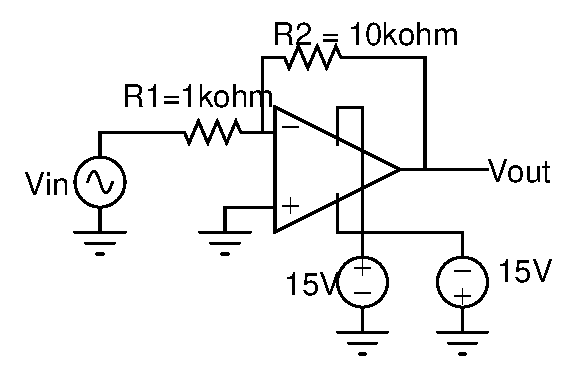
\includegraphics[scale = 1]{Exp_1_a.eps}
\end{figure}
\newpage
\subsection*{a.3 Simulation results}%[One more section] 
\begin{figure}[h!]
\centering
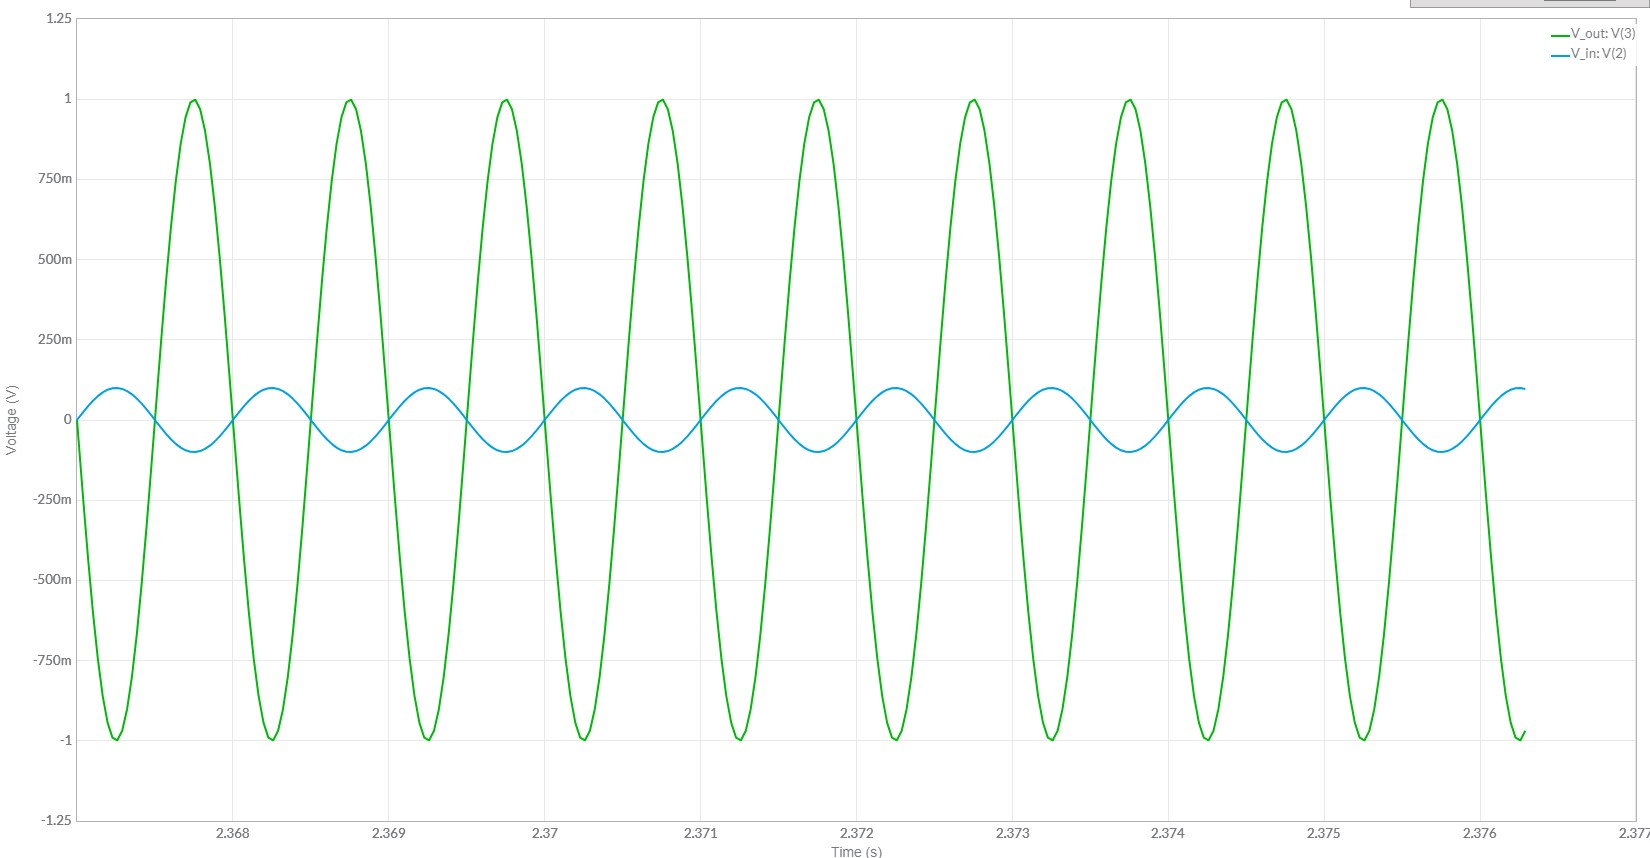
\includegraphics[scale = 0.4]{Sim_1_a.jpg}
\end{figure}

\subsection*{a.4 Experimental results}
\underline{\textit{Change the input amplitude from 0.1 V to 2 V and explain the observed output voltages:}}\\
When the input voltage signal equals 2V, the output should be \\(input voltage) * gain = 2 * 11 = 22 V. But since the supply voltage is \underline{+}15V, the output voltage reaches a maximum of 15 Volts. As we increase the input voltage supply, the output voltage begins to cut off at around 1.6V of input voltage.\\

\subsection*{a.5 Experiment completion status}
The experiment was completed during lab hours and the hand written report for the same was also submitted during lab hours.



%----------------------------------------------------------------------------------------------
%----------------------------------------------------------------------------------------------

\newpage

\addcontentsline{toc}{section}{Unnumbered Section}
\section*{(b) Differentiator}

\subsection*{b.1 Aim of the experiment}
The experiment aims to understand the behaviour of a differentiator circuit and also focuses on the effect of adding capacitor parallel to the resistor.

\subsection*{b.2 Design}
The design consists of an OpAmp with a feedback resistor connected between the output and the inverting input of the OpAmp and the input voltage is connected to the inverting input of the OpAmp with a capacitor between the input voltage and the input of the inverting pin of OpAmp. The output voltage $V_{o}$ of the circuit is given by:

 \begin{equation}
     V_{o} = - {RC} \cdot \frac{dV_{i}}{dt}
 \end{equation}     
 where the value of R = 10k$\Omega$, C = 0.01$\mu$F and the input is a triangular wave (\underline{+}2V, 2.5kHz).
 
\begin{figure}[h!]
\centering
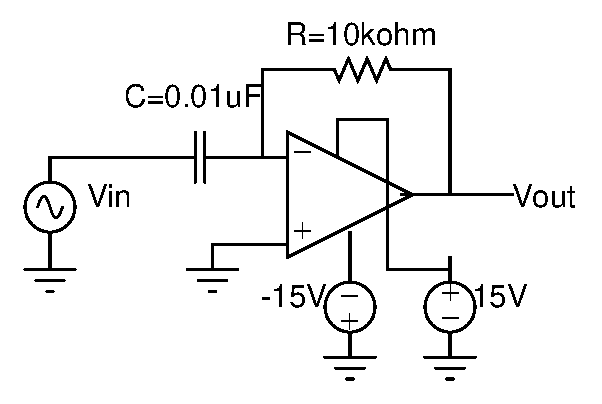
\includegraphics[scale = 1]{Exp_1_b_1.eps}
\end{figure}

\begin{figure}[h!]
\centering
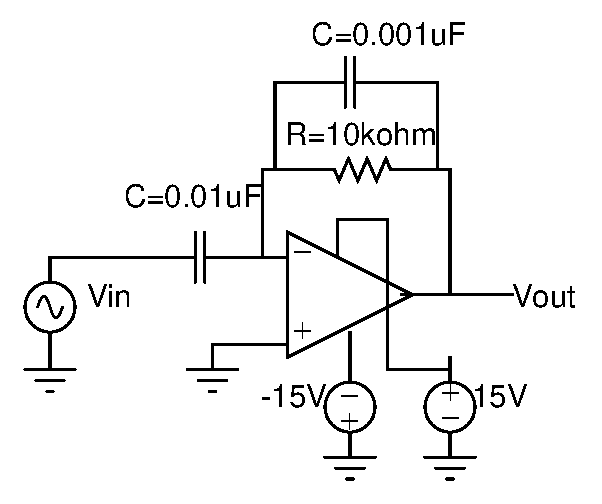
\includegraphics[scale = 1]{Exp_1_b_2.eps}
\end{figure}

\newpage
\subsection*{b.3 Experimental results}

\textbf{\underline{\textit{Observe the output waveform:}}}\\
The given circuit is a differentiator circuit which differentiates the input voltage and scales by a factor of R$\cdot$C in addition to inverting it. Since our input wave is a triangular wave, the output comes out to be a square wave. \\

\!\!\!\!\!\!\!\!\!\textbf{\underline{\textit{Connect small capacitor(0.001µF) in parallel with R, and observe output:}}}\\
The capacitor connected in parallel with the resistor stores the extra charge which is supplied by the current, and since the resistor no longer holds this extra charge, the output waveform is less noise as this capacitor dampens the noise.\\
\newpage
\subsection*{b.4 Simulation results}%[One more section] 
\begin{figure}[h!]
\centering
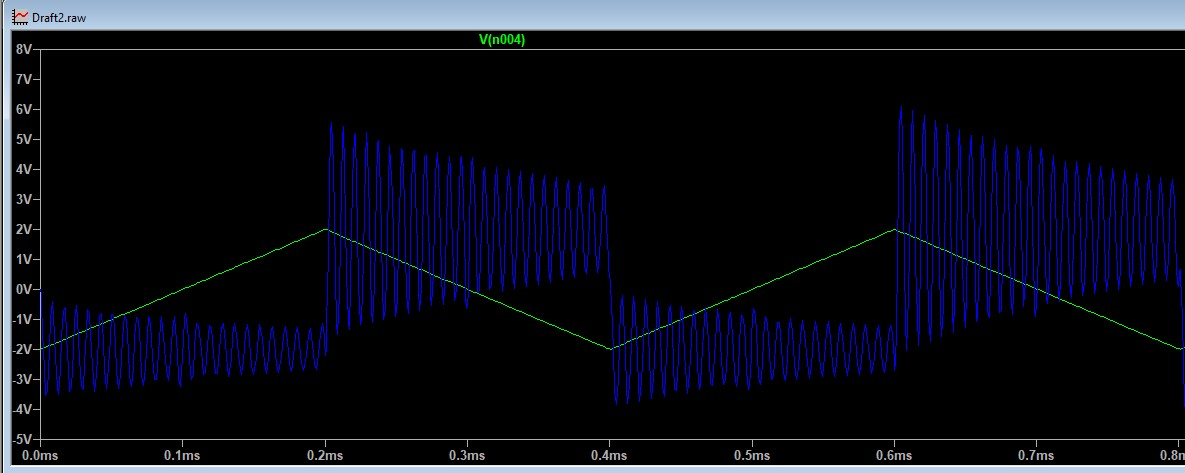
\includegraphics[scale = 0.4]{Sim_1_b_1.jpg}
\end{figure}

\begin{figure}[h!]
\centering
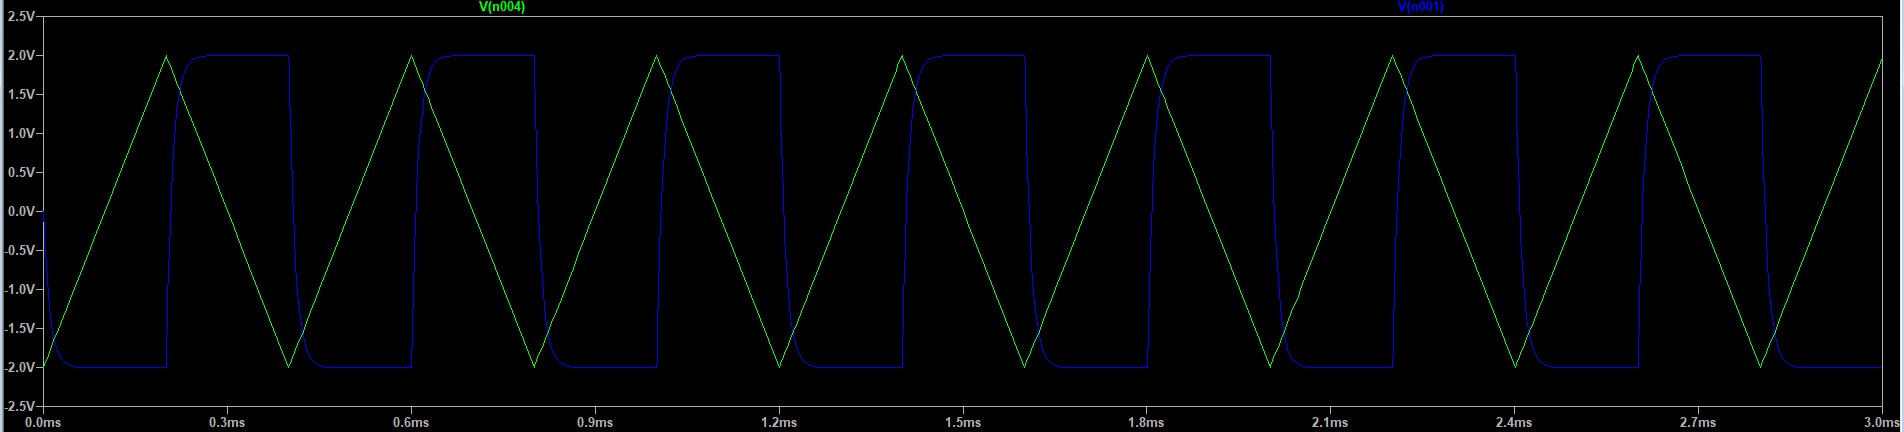
\includegraphics[scale = 0.6]{Sim_1_b_2.jpg}
\end{figure}

\subsection*{b.5 Experiment completion status}
The experiment was completed during lab hours and the hand written report for the same was also submitted during lab hours.
 %------------------------------------------------------------------------------------------
 %------------------------------------------------------------------------------------------

\newpage

\addcontentsline{toc}{section}{Unnumbered Section}
\section*{(c) Summer Amplifier Circuit}

\subsection*{c.1 Aim of the experiment}
The experiment aims to design a summer circuit which gives the output voltage as $V_{o}$=-2($X_{2}$+$X_{1}$/2) where $X_{1}$ and $X_{2}$ are the input voltages.

\subsection*{c.2 Design}
A resistor is connected between the inverting terminal and the output terminal of the OpAmp and we also connect a sets of resistor and input source in parallel across ground and inverting input. 
The equation below gives the general formula for gain in an inverting amplifier with $R_{2}$ being connected across the inverting input terminal and the output of the OpAmp and $R_{1}$ is connected between the input and inverting input of the OpAmp:
 \begin{equation}
     V_{o} = - V_{i}\cdot\frac{R_{2}}{R_{1}}
 \end{equation}     
 
 \begin{figure}[h!]
\centering
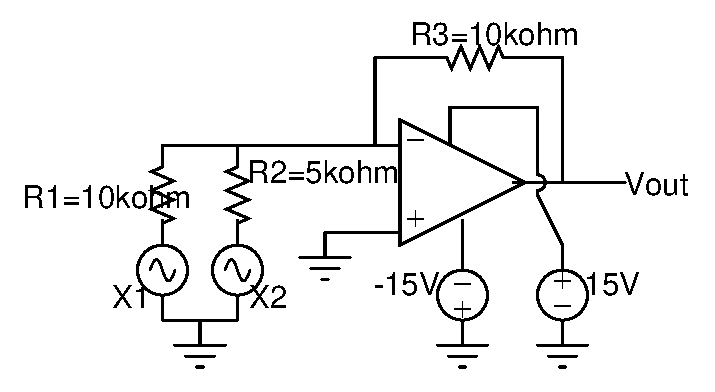
\includegraphics[scale = 1]{Exp_1_c.eps}
\end{figure}

 Simplifying the circuit we get the following expression for the output voltage:
 \begin{equation}
     V_{o} = - \frac{R_{3}}{R_{1}} \cdot (X_{1} + X_{2} \cdot \frac{R_{2}}{R_{1}} )
 \end{equation}
 In our case, the we are equipping the input $X_{1}$ with 4$V_{pp}$ voltage signal and the input $X_{2}$ with 2$V_{pp}$ amplitudes and frequency of 500Hz. 


\subsection* {c.3 Experimental results}
\underline{\textit{Design the values of $R_{1}$, $R_{2}$ and $R_{3}$:}}\\
Comparing the equation (4) with the given expression for the output voltage we come to following conclusions about the value of the resistances:\\
$R_{3}$ = 2*$R_{1}$, $R_{1}$ = 2*$R_{2}$ and $R_{1}$ = $R_{3}$. \\
Based on the value of resistances available to us we choose the value of $R_{1}$ and $R_{3}$ to be 10k$\Omega$ and that of $R_{2}$ to be 5k$\Omega$.


\!\!\!\!\!\!\!\!\!\underline{\textit{Comment on output voltage and $X_{1}$:}}\\
By substituting the given values of $X_{1}$ and $X_{2}$ in equation (4), we get the output voltage as 8$V_{pp}$ and phase shifted by $\pi$ radians. From equation (4), it can be seen that if we consider only the values of $X_{1}$ and $V_{o}$, we can see that, $V_{o}$=-2*$X_{1}$ and the same can also be seen in the simulation.
\newpage
\subsection*{c.4 Simulation results}%[One more section] 
\begin{figure}[h!]
\centering
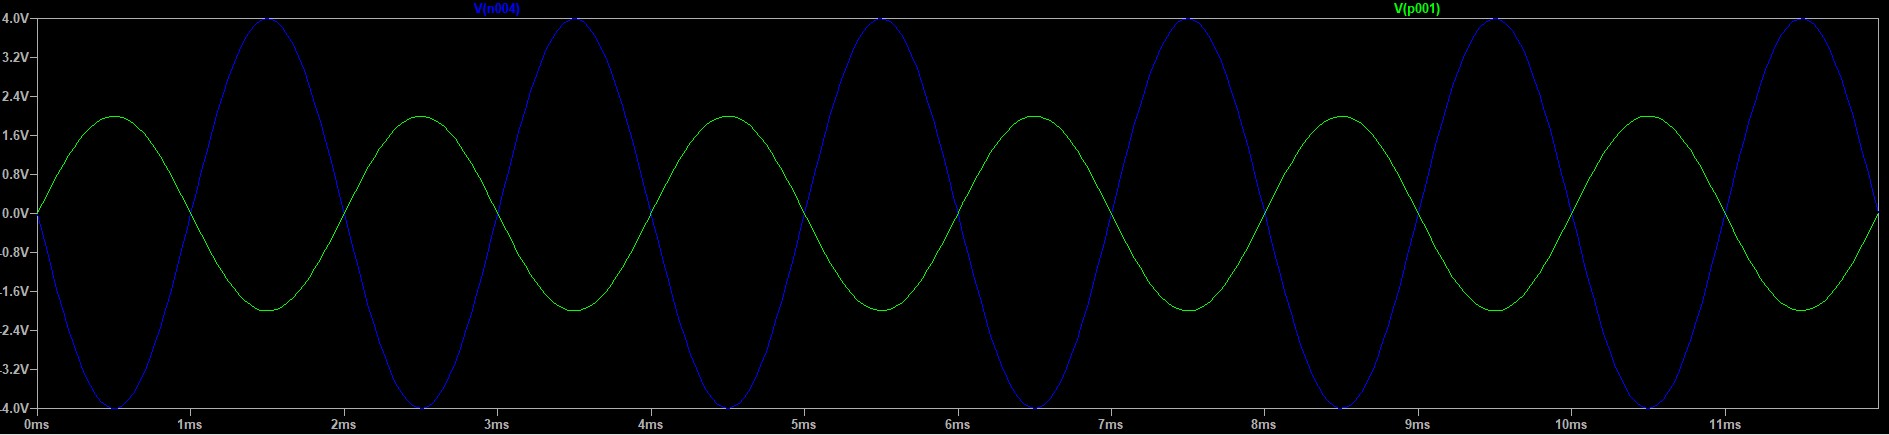
\includegraphics[scale = 0.6]{Sim_1_c.jpg}
\end{figure}

\subsection*{c.5 Experiment completion status}
The experiment was completed during lab hours and the hand written report for the same was also submitted during lab hours.

 %--------------------------------------------------------------------------------------
 %--------------------------------------------------------------------------------------




\newpage

\section*{(d) Equation Solver}
\subsection*{d.1 Aim of the experiment}
The experiment deals with the design and analysis of an equation solver where the output voltage is a function of the input voltage and our task is to design a certain to solve the equation. 

\subsection*{d.2 Design}
The output voltage is given by the following equation:
 \begin{equation}
     V_{o} = - (0.0001\cdot\frac{d}{dt}\cdot X_{1} + 2\cdot X_{2})
 \end{equation}     
 where the input values of $X_{1}$ in our case is $10\cdot\sin(2*\pi*500*t)$ and that of $X_{1}$ is $2.5\cdot\sin(2*\pi*500*t)$.

\begin{figure}[h!]
\centering
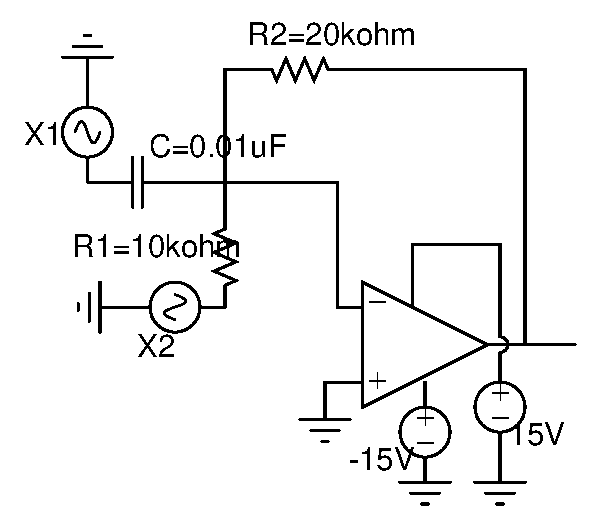
\includegraphics[scale = 1]{Exp_1_d.eps}
\end{figure}
\newpage
\subsection*{d.3 Simulation results}%[One more section] 
\begin{figure}[h!]
\centering
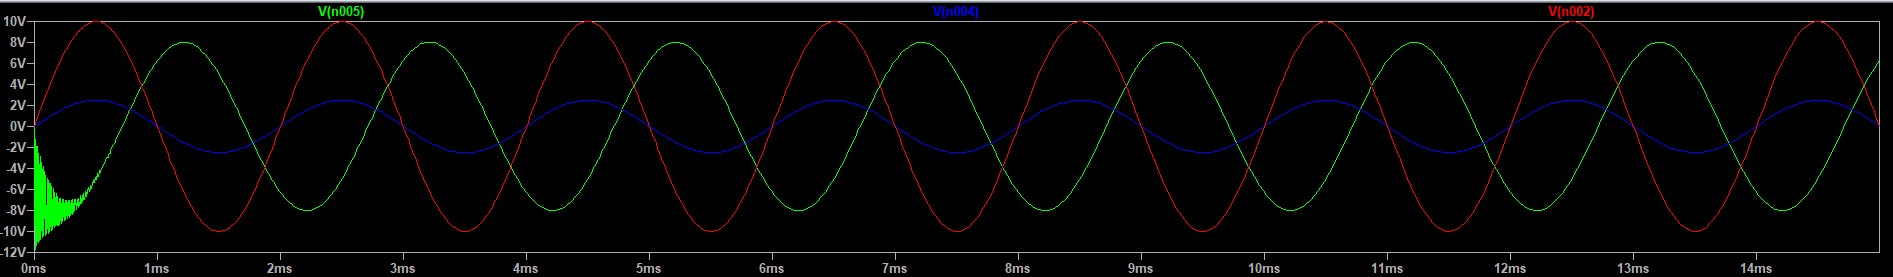
\includegraphics[scale = 0.6]{Sim_1_d.jpg}
\end{figure}


\subsection*{d.4 Experimental results}
\underline{\textit{Derive the expression of the expected output:}}\\
Substituting $X_{1}$=$a\cdot\sin(\omega\cdot t)$ and $X_{2}$=$b\cdot\sin(\omega\cdot t)$ in equation(4), we get\\
$V_{o}$ = - $(0.0001 \frac{d}{dt}(a\cdot\sin(\omega\cdot t) + 2\cdot b\cdot\sin(\omega\cdot t))$\\
$V_{o}$ = - $(0.0001 a\cdot\omega\cdot\cos(\omega\cdot t) + 2\cdot b\cdot\sin(\omega\cdot t))$\\
$V_{o}$ = - $(\sqrt{{a^2}\cdot{\omega^2}\cdot{10^{-8}}}\cdot\sin(\omega + \arctan(\frac{2\cdot b}{a\cdot\omega}\cdot 10^4)$\\
substituting the actual values of $X_{1}$ and $X_{2}$, we get,\\
$V_{o}$ = - $5.9 \cdot \sin(2\cdot\pi\cdot500\cdot t + 0.304)$\\

\subsection*{d.5 Experiment completion status}
The experiment was completed during lab hours and the hand written report for the same was also submitted during lab hours.
%----------------------------------------------------------------------------------------
%----------------------------------------------------------------------------------------
%----------------------------------------------------------------------------------------
%----------------------------------------------------------------------------------------

\newpage
\section{OpAmp Based Positive Feedback Circuits}
\section*{a. Schmitt Trigger Circuit}
\subsection*{a.1 Aim of the experiment}
The experimet aims to construct and study a schmitt trigger circuit based on the given values of $V_{TH}$, $V_{TL}$ and $V_{a}$\\
\subsection*{a.2 Design}
The general equation for the output voltage given $V_{o}$, $V_{in}$, $R_{1}$ and $R_{2}$ is:
 \begin{equation}
     V_{o} = V_{in} \cdot (1 + \frac{R_{1}}{R_{2}}) - V_{a}\cdot(\frac{R_{1}}{R_{2}})
 \end{equation}  
The equations to find $V_{TH}$ and $V_{TL}$ are listed below:
 \begin{equation}
     V_{TH} = \frac{V_{a} R_{1} + V_{DD} R_{2}}{R_{1} + R_{2}}
 \end{equation}   
 \begin{equation}
     V_{TL} = \frac{V_{a} R_{1} + V_{CC} R_{2}}{R_{1} + R_{2}}
 \end{equation}   
 The given value of $V_{TH}$ is +2.5V, $V_{TL}$ is -2.5V, $V_{DD}$ is 15V, $V_{CC}$ is -15V and a sinusoidal input of 10$V_{pp}$ with 1kHz frequency is applied.
  
\begin{figure}[h!]
\centering
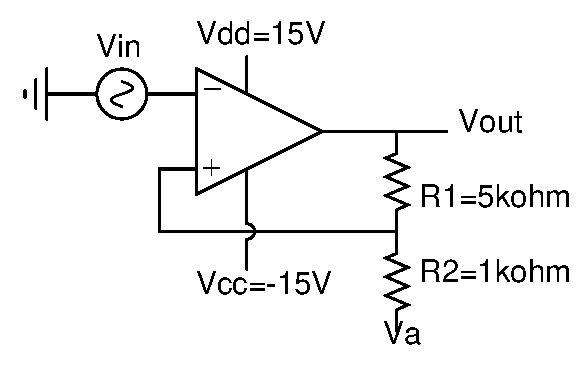
\includegraphics[scale = 1]{Exp_2_a.eps}
\end{figure}

\begin{figure}[h!]
\centering
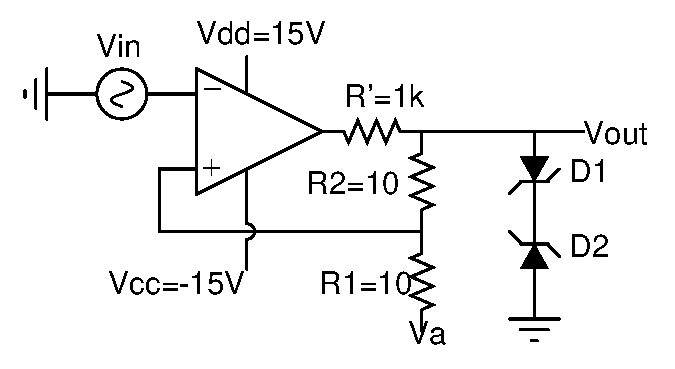
\includegraphics[scale = 1]{Exp_2_b.eps}
\end{figure}

% \subsection*{a.3 Simulation results}%[One more section] 
% \begin{figure}[h!]
% \centering
% \includegraphics[scale = 0.4]{Exp_5_1_simulation.jpg}
% \end{figure}


\subsection*{a.3 Experimental results}
\underline{\textit{Design the schmitt trigger based on the values given:}}\\
Upon substituting the correct values in equation(7), we get the relation between $R_{1}$ and $R_{2}$ as $R_{1}$ = 5 * $R_{1}$\\
Based on the availability in lab resistors of 1k$\Omega$ and 10k$\Omega$ were used and $R_{1}$ was chosen to be 5k$\Omega$ and $R_{2}$ was chosen to be 1k$\Omega$.
\underline{\textbf{(i) Keeping $V_{a}$ = 0V:}}\\
 \begin{table}[!hbt]
		\begin{center}
		\begin{tabular}{|c|c|c|c|} \hline
			& $V_{o} (peak to peak)$ & $V_{TH}$ & $V_{TL}$ \\ \hline
			Expected & 30 & 2.5 & -2.5 \\ \hline
            Observed & 28.60 & 2.72 & - 2.75 \\ \hline 
		\end{tabular}
		\end{center}
\end{table}

\underline{\textbf{(ii) Keeping $V_{a}$ = 2V:}}\\
On substituting the values of $V_{DD}$, $V_{CC}$, $R_{1}$ and $R_{2}$ in equations(7) and (8), we get the value of $V_{TH}$ as 4.166V and that of $V_{TL}$ as -834 mV.\\
 \begin{table}[!hbt]
		\begin{center}
		\begin{tabular}{|c|c|c|c|} \hline
			& $V_{o} (peak to peak)$ & $V_{TH}$ & $V_{TL}$ \\ \hline
			Expected & 30 & 4.17 & -0.834 \\ \hline
            Observed & 28.60 & 4.18 & -1.25 \\ \hline 
		\end{tabular}
		\end{center}
\end{table}

 \!\!\!\!\!\!\!\!\!\underline{\textit{Comment on this design of schmitt trigger and its feasibility:}}\\
No, this is not a robust design of Schmitt Trigger because the values of $V_{TH}$ and $V_{TL}$ are dependent on the values of supply voltages.


\subsection*{a.4 Experiment completion status}
The experiment was completed during lab hours and the hand written report
for the same was also submitted during lab hours.

%----------------------------------------------------------------------------------------
%----------------------------------------------------------------------------------------
%----------------------------------------------------------------------------------------
%----------------------------------------------------------------------------------------

\section*{b. Modified Schmitt Trigger Circuit}
\subsection*{b.1 Aim of the experiment}
The experiment aims to construct and study a modified schmitt trigger circuit (consisting of an extra resistor and two Zener diodes)\\
\subsection*{b.2 Design}
The general equation for the output voltage given $V_{o}$, $V_{in}$, $R_{1}$ and $R_{2}$ is:
 \begin{equation}
     V_{o} = R_{1} \cdot (V_{in}\cdot(\frac{1}{R_{1}} + \frac{1}{R_{2}} - V_{a})
 \end{equation}  
The equation to find $V_{TH}$ is:
 \begin{equation}
     V_{TH} = (\frac{V_{CC}}{R_{1}} + V_{a}) \cdot (\frac{R_{1}\cdot R_{2}}{R_{1} + R_{2}})
 \end{equation}   
 The equation to find $V_{TL}$ is:
 \begin{equation}
     V_{TL} = (\frac{V_{DD}}{R_{1}} + V_{a}) \cdot (\frac{R_{1}\cdot R_{2}}{R_{1} + R_{2}})
 \end{equation}   
 
% \begin{figure}[h!]
% \centering
% \includegraphics[scale = 0.4]{Exp_5_design.jpg}
% \end{figure}


% \subsection*{a.3 Simulation results}%[One more section] 
% \begin{figure}[h!]
% \centering
% \includegraphics[scale = 0.4]{Exp_5_1_simulation.jpg}
% \end{figure}


\subsection*{b.4 Experimental results}
\underline{\textit{Explain the purpose of $R^'$ and what will happen if the value of $R^'$ becomes 0:}}\\
The resistor $R^'$ helps in keeping a check on the current that is flowing through the zener diode. A higher current will damage the diode. The resistor keeps a check on that and if we don't use any resistor then our device maybe at risk.\\

\!\!\!\!\!\!\!\!\!\underline{\textit{Compare the theoretical and experimental values of $V_{TH}$ and $V_{TL}$:}}\\
The experiment was completed during lab hours and the hand written report for the same was also submitted during lab hours.\\
\newpage
 \begin{table}[!hbt]
		\begin{center}
		\begin{tabular}{|c|c|c|c|} \hline
			& $V_{o} (peak to peak)$ & $V_{TH}$ & $V_{TL}$ \\ \hline
			Expected & 2 p & $\frac{p}{2}$ & $\frac{-p}{2}$ \\ \hline
            Observed & 10.20 & 3.2 & -3 \\ \hline 
		\end{tabular}
		\end{center}
\end{table}
\!\!\!\!\!\!\!\!\!where p=reverse bias drop + forward bias drop of zener diode = 4.7+0.7=5.4V
\!\!\!\!\!\!\!\!\!It can be clearly seen that the addition of zener diodes makes the schmitt trigger more robust than the previous part.

\subsection*{b.5 Experiment completion status}
The experiment was completed during lab hours and the hand written report for the same was also submitted during lab hours.


%----------------------------------------------------------------------------------------
%----------------------------------------------------------------------------------------
%----------------------------------------------------------------------------------------
%----------------------------------------------------------------------------------------

\newpage
\section{OpAmp based feedback circuit}
\subsection{Aim of the experiment}
Determine the type of feedback circuit and observe its effect on the output waveform.
\subsection{Design}
The below equation governs the circuit:
 \begin{equation}
     V_{+} - V_{-} = \beta V_{o} - \alpha V_{in}
 \end{equation}  
where $\beta$ is given by:
 \begin{equation}
     \beta = \frac{R_{4}}{R_{3} + R_{4}} - \frac{R_{1}}{R_{1} + R_{2}}
 \end{equation}   
 and $\alpha$ is given by:
 \begin{equation}
     \alpha = \frac{R_{2}}{R_{1} + R_{2}}
 \end{equation}   
 The type of feedback depends on the sign of $\beta$, if $\beta$ is positive then so is feedback and if $\beta$ is negative then the feedback is alos negative.
 
\begin{figure}[h!]
\centering
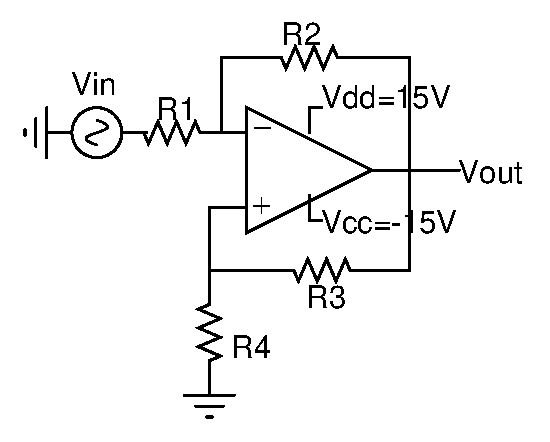
\includegraphics[scale = 1]{Exp_3.eps}
\end{figure}


% \subsection*{a.3 Simulation results}%[One more section] 
% \begin{figure}[h!]
% \centering
% \includegraphics[scale = 0.4]{Exp_5_1_simulation.jpg}
% \end{figure}


\subsection{Experimental results and Simulation}
\underline{\textbf{i) ${R_{1}}$ = 1k$\Omega$, $R_{2}$ = 10k$\Omega$, $R_{3}$ = 100k$\Omega$ and $R_{4}$ = 1k$\Omega$:}}\\
Using equation(13), we can calculate the $\beta$ to be $- \frac{90}{1111} < 0$, hence the circuit is negative feedback.\\
\!\!\!\!\!\!\!\!\!\underline{\textit{Experimental verification:}}\\
$V_{out}$ is a sinusoidal wave with 2.16V peak to peak amplitude, 1kHz frequency and out of phase with the input.\\

\!\!\!\!\!\!\!\!\!\underline{\textbf{ii) ${R_{1}}$ = 1k$\Omega$, $R_{2}$ = 100k$\Omega$, $R_{3}$ = 10k$\Omega$ and $R_{4}$ = 1k$\Omega$:}}\\
Using equation(13), we can calculate the $\beta$ to be $\frac{90}{1111} < 0$, hence the circuit is positive feedback.\\
\!\!\!\!\!\!\!\!\!\underline{\textit{Experimental verification:}}\\
$V_{out}$ is a waveform with the OpAmp going into saturation with $V_{out}$ = 27.4V peak to peak.\\


\subsection{Experiment completion status}
The experiment could not be completed during lab hours.

\end{document}

